\documentclass[10pt,twocolumn]{article}
\usepackage[a4paper, left=1.5cm, right=1.5cm, top=2cm, bottom=3cm]{geometry}
\usepackage[T1]{fontenc}
\usepackage[utf8]{inputenc}
\usepackage[italian]{babel}
\usepackage{amsmath}
\usepackage{titling}
\usepackage{caption}
\usepackage{graphicx}
\usepackage{float}
\usepackage{relsize}
\usepackage{amsmath}
\usepackage{sectsty}
\usepackage{ragged2e}
\usepackage{circuitikz}
\usepackage{booktabs}
\usepackage{enumitem}
\usepackage{tikz}
\usepackage{physics}
\usepackage{xcolor}
\usepackage[most]{tcolorbox}
\usepackage{tikz-3dplot}
\usepackage{tikz}
\usepackage{ragged2e}
\usepackage{siunitx}
% \usepackage{booktabs}
\usepackage[colorlinks=true, linkcolor=black]{hyperref}  %per rendere l'indice genrale "interattivo"
\usepackage{enumitem}  %distanza degli itemize
\setlist[itemize]{itemsep=4pt, parsep=1pt}
\newtcolorbox{nota}{
  blanker,
  before skip=1em,
  after skip=1em,
  left=1em,
  borderline west={1pt}{0pt}{black},
  fontupper=\itshape,
  before upper={\noindent\textbf{Nota}:\quad}
}



\begin{document}
\justifying
	\title{\textbf{Misura della curva caratteristica del diodo}}
	\author{Brusini Alessio \hspace{0.7cm} Ferrari Carola \hspace{0.7cm} Mirolo Manuele \hspace{0.7cm} Stroili Emanuele}
	\date{21 Ottobre 2025}
	\maketitle
	\newgeometry{left=3cm, right=3cm, top=4cm, bottom=4cm}
	\onecolumn
\vspace{3cm}
	\begin{abstract}
		\centering
		\large
    L'esperimento consiste nell'ottenere la curva caratteristica del diodo, linealizzarla in scala semilogaritmica, 
	fare un fit e, tramite un'analisi dei dati: ricavare il coefficente $\eta$ caratteristico del diodo a diverse temperature
	e individuare il valore del voltaggio build-in ($V_0$) del diodo

       
	\end{abstract}

	\newpage
\restoregeometry
\twocolumn

\begin{figure}[H] % [h] = here, posizione approssimativa
  \centering
  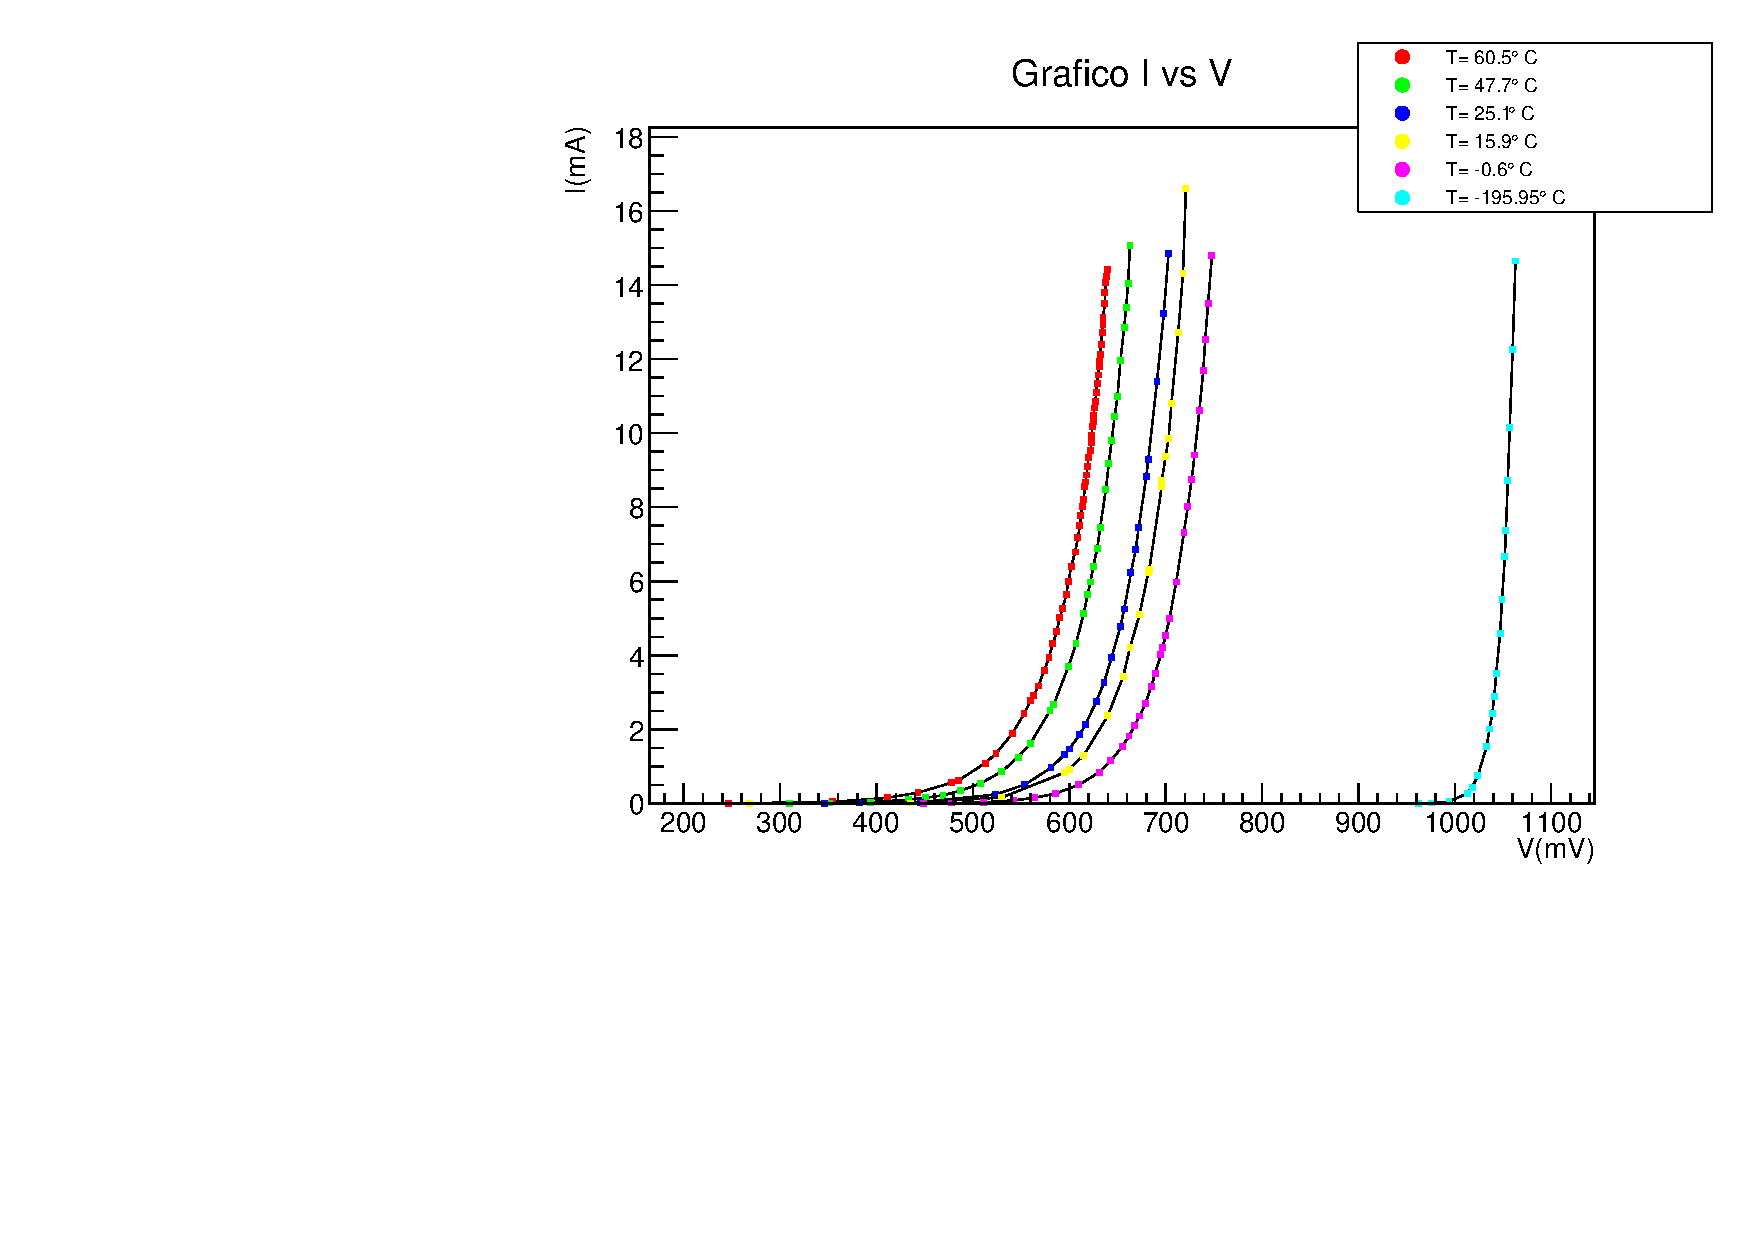
\includegraphics[width=0.5\textwidth]{I_vs_V.pdf} % o .png, .pdf, ecc.
  \label{fig:II}
\end{figure}
Il primo grafico che viene presentato mostra l'andamento della corrente $I$ in funzione del voltaggio $V$ a diverse 
temperature. In questo grafico osserviamo che la curva caratteristica del diodo presenta un comportamento esponenziale, 
che verifica la formula che si trova in letteratura per un diodo ideale:
\[
\displaystyle I(V)= I_0 e^{(\frac{qV}{\eta kT})} - 1
\]
Si può notare come, al diminuire della temperature:

\begin{itemize}
  \item la derivata prima aumenti
  \item l'innalzamento si verifica a valori di di $V$ sempre maggiori
\end{itemize}
La seconda considerazione ci fa intuire che il passaggio della corrente sia estremamente condizionato dalla temperature, questo perchè 
a temperature minori vi sarà una minore eccitazione degli elettroni, conseguentemente, per oltrepassare la barriera di potenziale della giunzione
essi avranno bisogno in voltaggio maggiore.


\begin{figure}[H] % [h] = here, posizione approssimativa
  \centering
  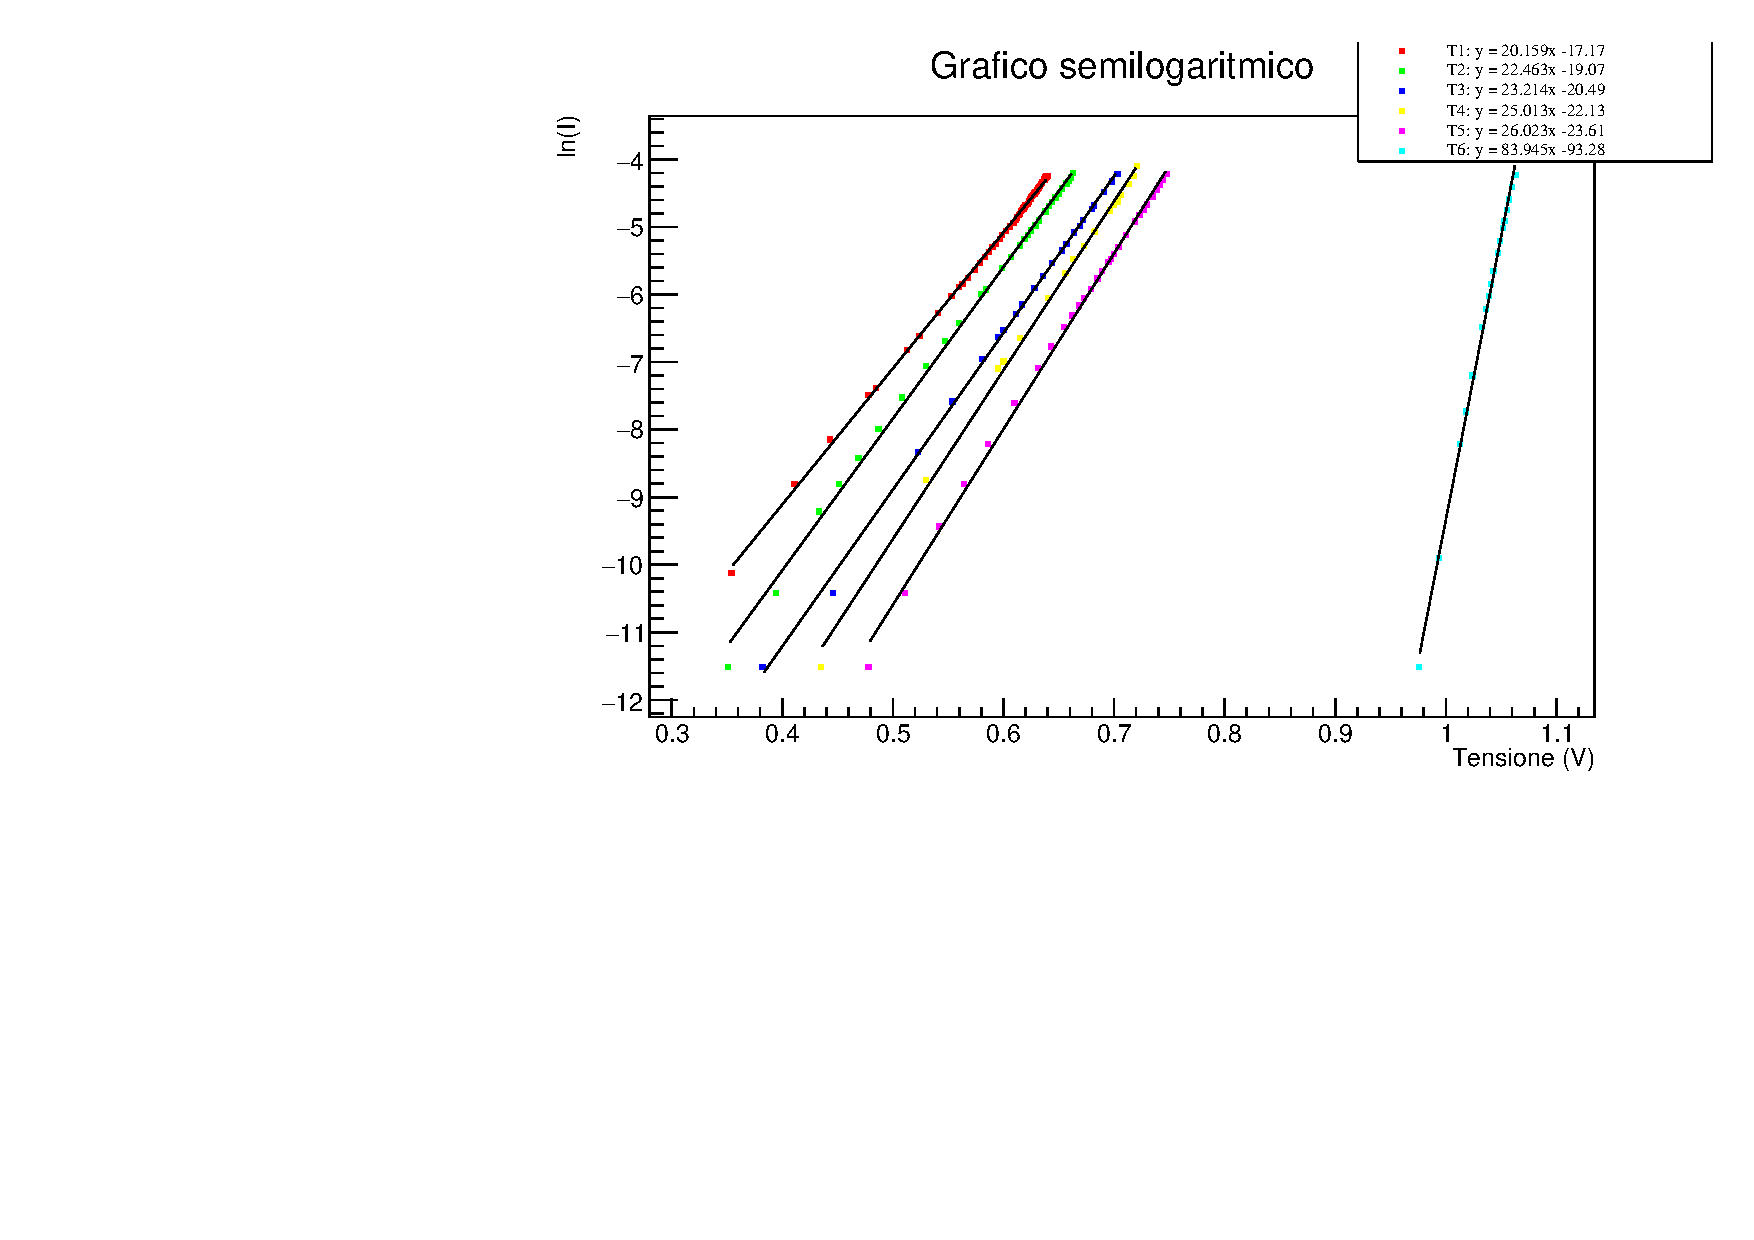
\includegraphics[width=0.5\textwidth]{scala_semilogaritmica.pdf} % o .png, .pdf, ecc.
  \label{fig:I_V_}
\end{figure}
Ivi è riportato il grafico della curva caratteristica del diodo in scala semilogaritmica,
su cui è stato fatto il fit lineare. 
Tramite esso siamo riusciti a ricavare il valore di $\eta$, 
caratteristico per diverse temperature.

\begin{table}[H]
	\centering
	\begin{tabular}{|c|c|}
		\hline
		\textbf{T} [$^\circ$C] & \textbf{$\eta$} \\ \hline
    60.5 & 1.702 \\ \hline
    47.7 & 1.604 \\ \hline
    25.1 & 1.676 \\ \hline
    -0.6 & 1.637 \\ \hline
    -195.5 & 1.791 \\ \hline
	\end{tabular}
\end{table}
Si può notare che l'ultimo fit, quello svolto a temperature minore (azoto liquido), presenta un valore di $\eta$  più alto,

\begin{figure}[H] % [h] = here, posizione approssimativa
  \centering
  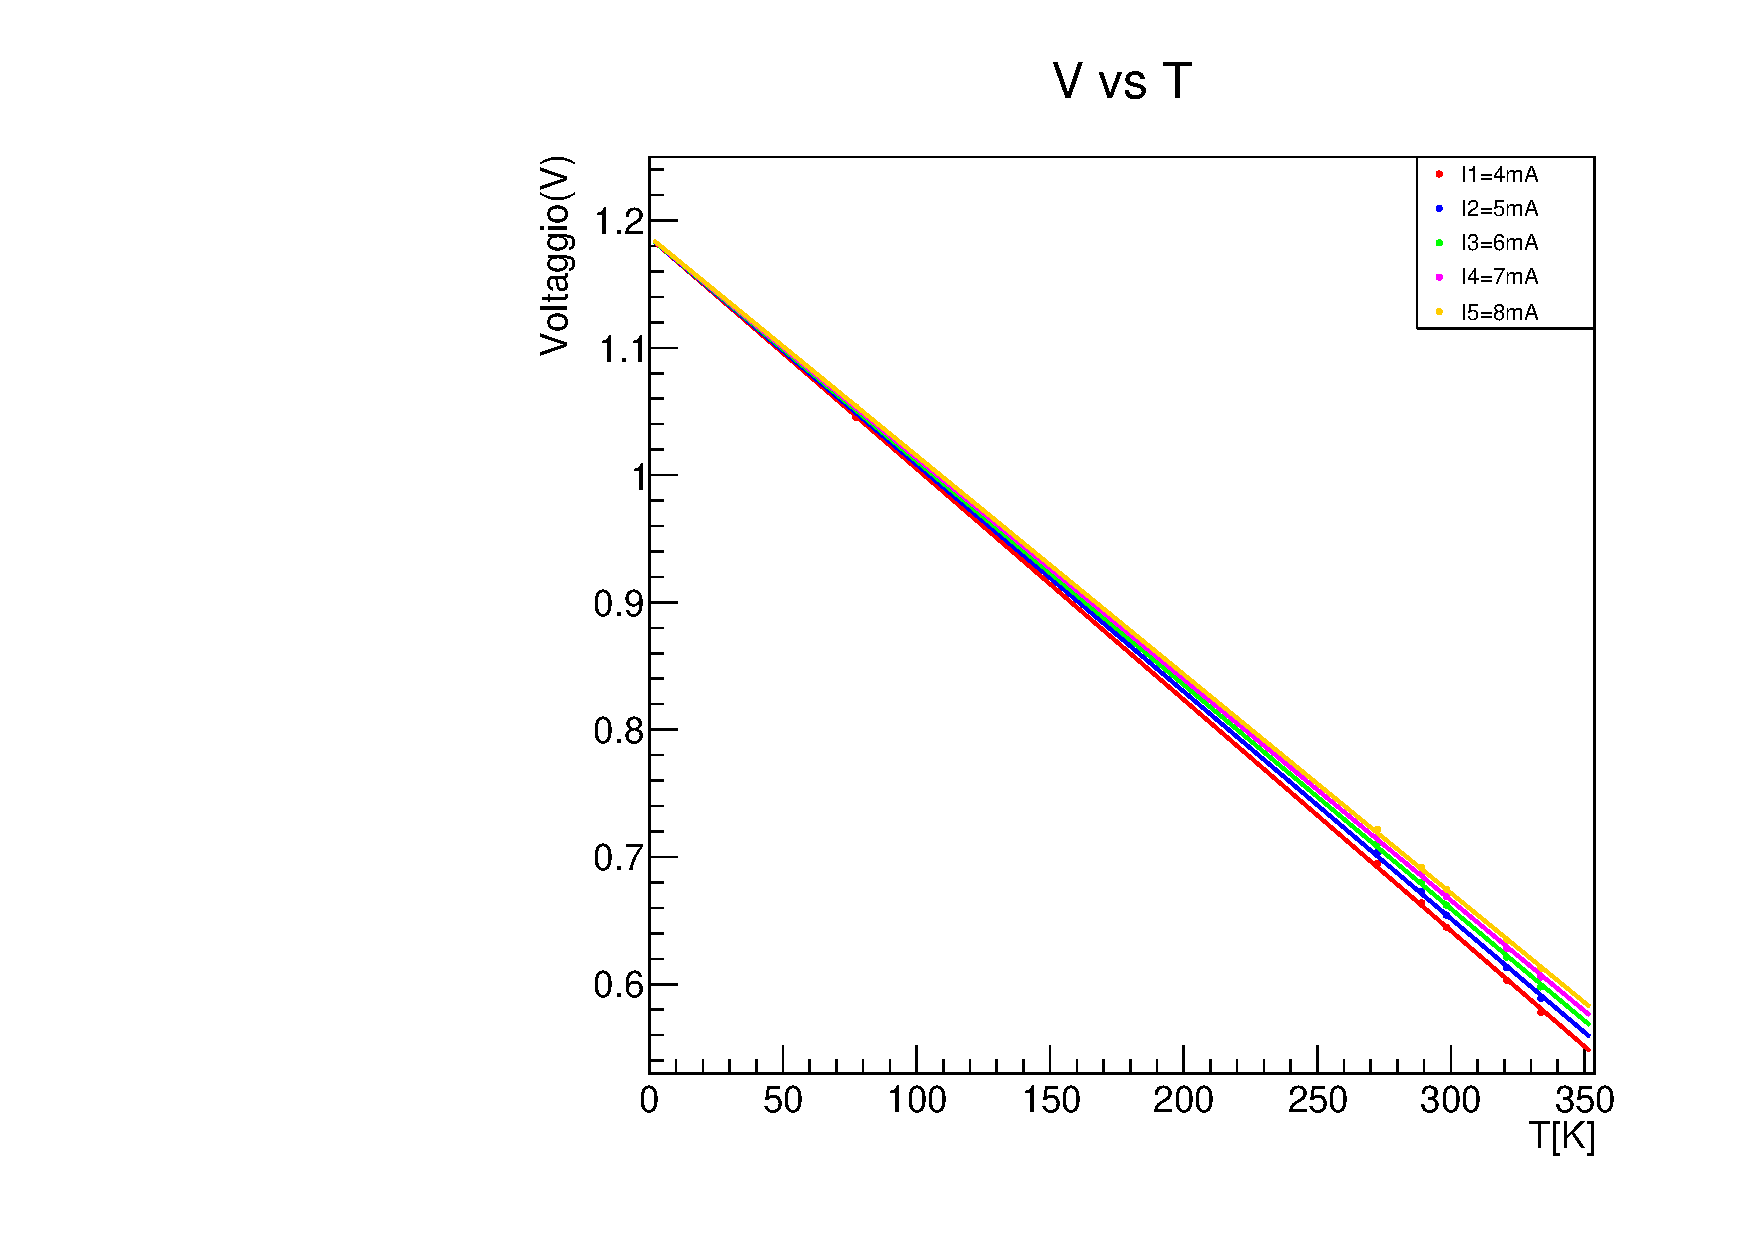
\includegraphics[width=0.5\textwidth]{V_vs_T.pdf} % o .png, .pdf, ecc.
  \label{fig:V}
\end{figure}
Il grafico sopra riportato mostra l'andamento di V rispetto a T
per specifici valori di corrente, scelti accurandosi di essere ben sopra del ginocchio della curva caratteristica del diodo
e al contempo sotto la fine della curva.
Si nota come, al tendere a 0 della T il valore di V tenda anch'esso ad uno specifico valore (ciò è evidenziato dal primo grafico), che sarà il valore
di tensione di build-in del diodo. Nel nostro caso, tale valore si trovi nell'intervallo $[1.18V-1.20V]$
\begin{figure} [H]% [h] = here, posizione approssimativa
  \centering
  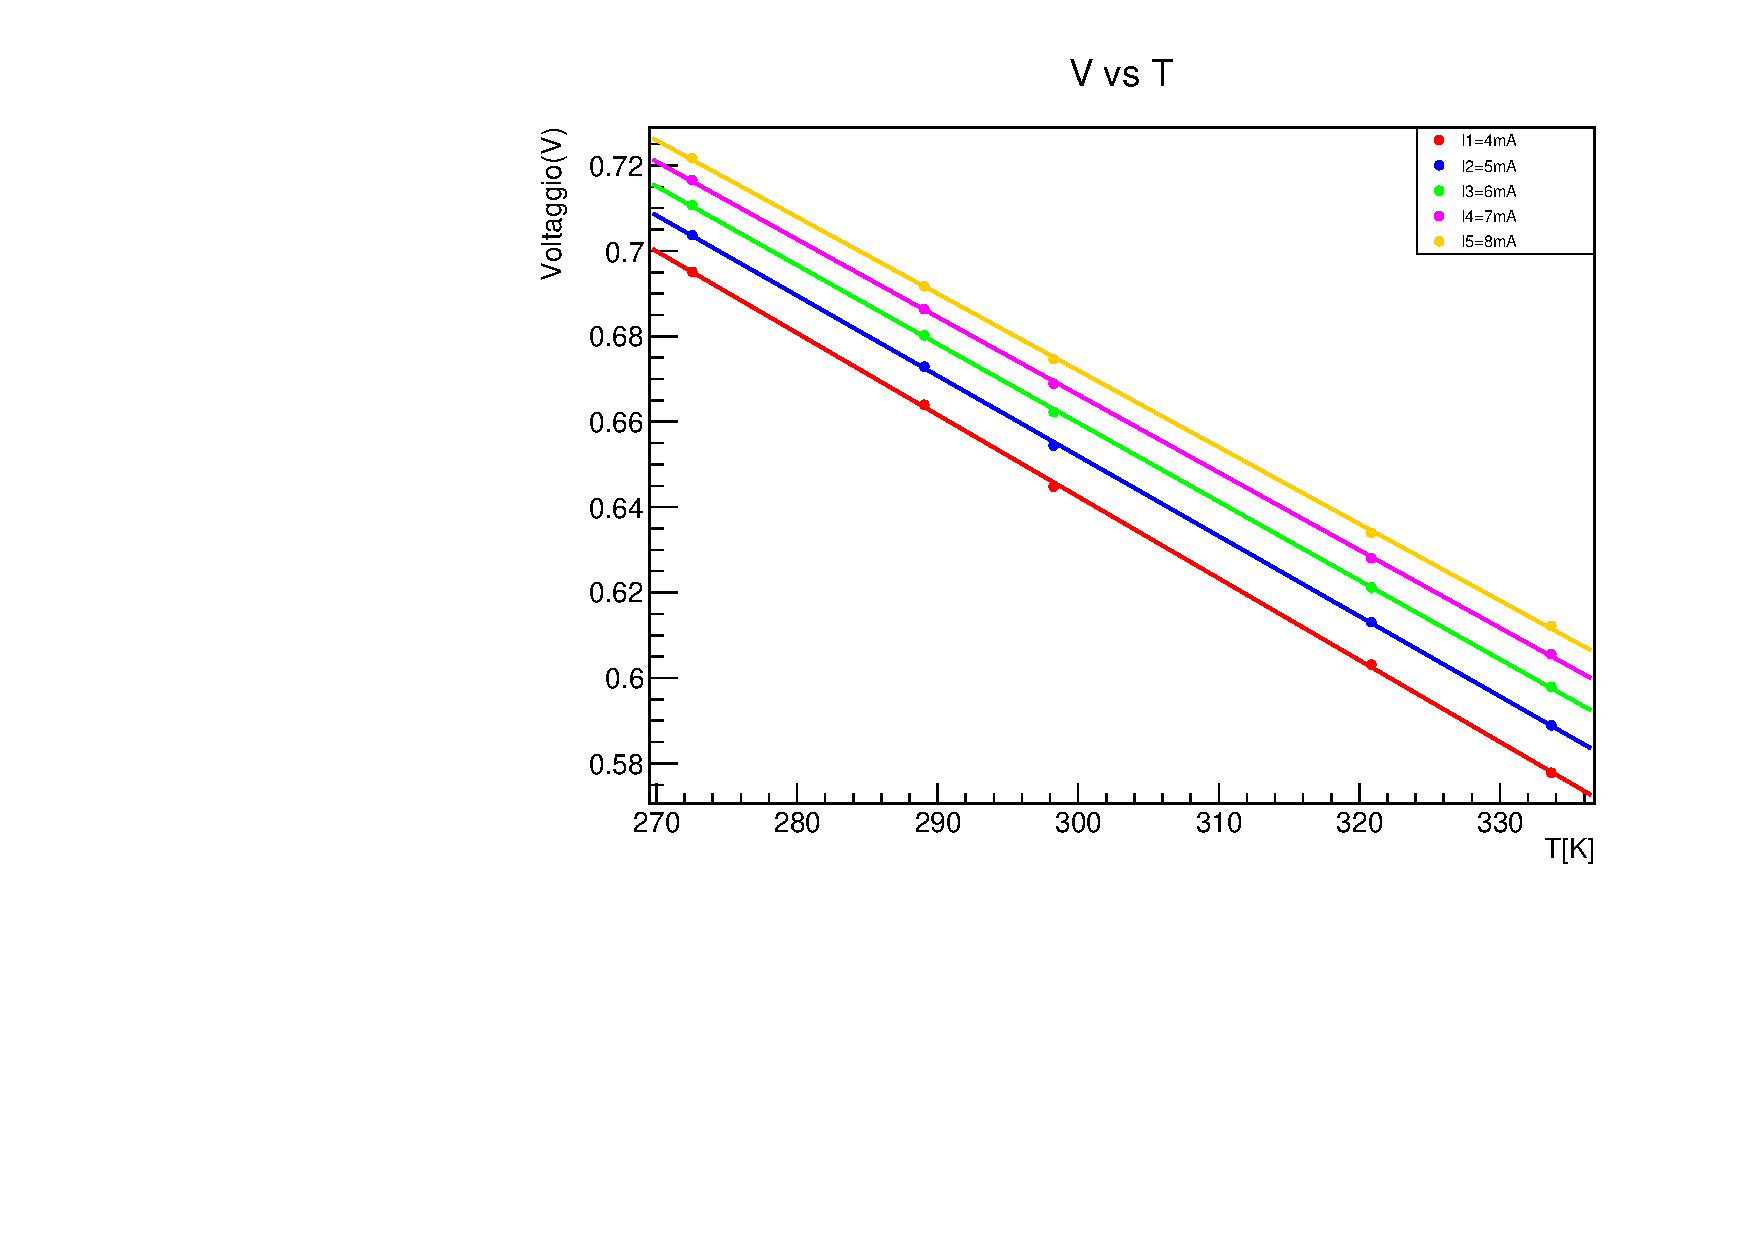
\includegraphics[width=0.5\textwidth]{V_vs_T_lim.pdf} % o .png, .pdf, ecc.
  \label{fig:V_I_}
\end{figure}

Quest'ultimo grafico viene riportato per evidenziare la bontà del fit svoltosi per i punti precedenti, 
nonostante il numero di punti disponibili per farlo non fosse elevato.

\end{document}